
\section*{\centering Abstract}
\small The extent to which electoral systems change legislative preference and representation remains debatable. This paper investigates how parties and legislators strategically position themselves in response to an institutional change using the case of Taiwan's electoral reform from the Single Non-transferable Vote (SNTV) to the Single-Member Districts (SMD). To this end, I apply dynamic ideal point estimation to measure legislators' ideological preferences and study whether the reform moderates the level of intraparty disagreement induced by the change in the systems. In this chapter, I provide compelling evidence that institutional change does influence the relationship between legislators and their general ideological preference in relation to their party and the opposite party. The empirical evidence shows that intraparty fractionalisation increases and ideological differences between major parties are drastically polarised in the SMD. Controlling for yearly effects during the presence of the reform, however, I find the impact of party division decreases as time goes by. This chapter complements mounting evidence that electoral systems play an important role in explaining lawmakers' preferences and the changes in ideological positioning, which sheds light on party polarisation and party competition in modern democracies.\footnote{An earlier version of the chapter was presented at the 2020 APSA, and I would like to thank Miguel Maria Pereira, Jon Fiva, and Daniel Smith for constructive feedback and suggestions. In addition, I gratefully thank the Centre for Legislative Studies at Soochow University for providing the historical roll-call data.}

\clearpage

\section*{\centering Introduction}
How electoral systems change party competition is key to understanding the theoretical development of party politics in the real world. The literature has envisioned ideological changes behind the influence of different electoral rules on party competition and representation \citep[e.g.][]{Curini2012, Dow2011, Ezrow2008}, while scholars have developed expert surveys \citep[][]{Bakker2014a, Benoit2006, Huber1995} and analyses of party manifestos \citep[][]{Budge2001, Budge1994, Huber1995, Volkens2013} to compare party ideological positions across time and across countries. Theoretical and empirical works have conceptually discussed merits and deficiencies of various electoral systems across countries \citep[e.g.][]{Andre2014, Cox2008, Shugart2003,  Burnham2005},\footnote{Among these, \citet{Cain1987, Grofman1999, Shugart2003, Ware2009, Colomer2011} are the most widely cited theoretical and empirical works.} whereas comparative studies, such as \citet{Carroll2019, Dow2011, Ezrow2008}, measure voters' party ideology and heterogeneity and examine differences across systems in multiple countries. While insightful for theoretical contribution on party politics, these studies only illustrate evidence by simply comparing political phenomenon under different systems but rarely looks at a system throughout pre- and post-reform periods in which two parties compete on a single dimension.

Recent decades saw reforms of electoral systems from the single non-transferable voting (SNTV) with multi-member districts system to single-member districts (SMD) in several East-Asian democracies (i.e. Japan, South Korea and Taiwan). These reforms naturally provide empirical evidence to casually examine the impact of electoral changes on inter-party divisions and legislators' relation with their own party. Previous studies have envisioned a number of potential reasons that explain why legislators position themselves differently under different electoral systems \citep{Catalinac2016} or electoral rules in mixed member electoral systems \citep[e.g. ][]{Batto2012, Hirano2011, Jun2010, Rich2014}. 

The core difference is thought to be district magnitude. Specifically, SNTV allows more than one candidate to be elected per district and leads to a dispersed distribution of within-party ideology along the spectrum. It has been criticised for creating excessive intraparty competition and chaos \citep[][]{Cox1990, Hirano2006, Ames1995}, as well as encouraging factional and candidate-centered electoral politics \citep[e.g.][]{Batto2016, Wu2003}. However, combining plurality rule with a single vote per voter, SMD fixes the district magnitude to one and is expected to mitigate intraparty competition \citep[][]{Carey1995, Shugart2003, Andre2014}. As the result, literature anticipates that under this system, electoral competition is winnowed down to two parties \citep[][]{Catalinac2016}. Under the vote-maximising strategy, both parties can capture the universe of votes on their respective sides of the spectrum and seek to win votes in between. Consequentially, candidates elected by SMD tend to converge to their opponent on a centrally located position along the spectrum.

Some earlier studies regarding past electoral reforms in Japan and Colombia \citep[e.g.,][]{Hideo1998, Crisp2002, Christensen1994} find weak association between electoral reforms and changes in candidates' behaviours, whereas recent research, for example, on the reform, finds the impact of electoral institutional changes not only decrease their incentives to run on a personal vote \citep[e.g.,][]{Catalinac2017, Sheng2014a} but converge their preference to the median on a single dimension as well \citep[e.g.,][]{Catalinac2017, Catalinac2016, Sheng2014a}. Thus, the finding in this chapter is inconsistent with the similar reform in Japan studied by \citet{Catalinac2016} that MPs converge in SMD but diverge in SNTV by analysing the election manifesto. With a more granulated data set on historic roll call, the evidence in this chapter shows that the reform in Taiwan temporarily dis-unified partisan distance and polarised both mainstream parties' distance when the reform occurred. 

In this chapter, I provide compelling evidence that institutional change does influence the relationship between legislators and their general ideological preference in relation to their party and the opposite party. First of all, I estimate individual legislator's ideological positions from roll call votes continuously covering pre- and post-reform periods. Expectation Maximisation (EM) algorithm is applied to a dynamic ideal point model to estimate each legislator's position from 1992 to 2015 at a session level, where individual recursively updates her prior of ideal point every session. Then, inter- and intraparty distance of ideological positions are constructed from the estimated positions. 

Therefore, econometric regressions are introduced to empirically examine the above two questions and find noticeable shifts in ideological positions after the reform.  Inter-party analysis suggests that in the electoral transition from SNTV to SMD, ideological positions between two major parties are drastically polarised. In the meanwhile, this electoral transition significantly dis-unifies co-partisan legislators on the ideological spectrum. As a result, I conclude that during the transition from SNTV to SMD, parties underwent a phase of ``disunited polarization'': co-partisans became ideologically disunited while the reform exacerbates inter-party division. These findings help clarify actual outcomes of the electoral reform through SNTV to SMD, shedding light on party polarisation and intraparty competition in modern democracies. 

\section*{\centering Legislators' Positions and Electoral Systems}
The arena of policy-making process in most democratic nations, such as Taiwan, is mainly dominated by elected legislators. Their political positionings and attitude can have real-life impact on different population groups with different socio- and economic-status. In general, the legislative votes made by legislators in each session is a reflection of their preference genuinely show their political intention and interests, whose information allows us to track their preference and attitude across time. Numerous studies have primarily been concentrated on the estimating party ideological positions from perspectives on comparative politics \citep[e.g.,][]{Carroll2019, Hix2009,Budge1994, Lo2014, Curini2012, Catalinac2016}, which is important in light of the explosion of interest in understanding party system development under different electoral systems. The link between the difference of electoral systems and party ideological position is important because it changes the attention legislators pay to constituents and electoral strategies candidates adopt during the election \citep[][]{Andre2015, Andre2014b, Catalinac2016, Fiva2020, Luor2008, Luor2009}. 

The development of the party system is inseparable from the design of electoral systems. The electoral systems with different sizes of district magnitudes, it has generally been argued, generate varying incentives for legislators to seek personal votes or strengthen a collective party reputation \citep[][]{Andre2015,Andre2015, Carey1995, Cox1997}. The SNTV-MMD system, for example, combining the plurality rule with a single vote per voter and a district magnitude larger than one, is known to increase intraparty competition \citep{Calvo2011, Cox1990, Reed2003, Carey1995, Merrill2002} and encourage heavy use of pork-barrel projects \citep[e.g.][]{Reed2005, Shugart2005, Hirano2006} as well as dirty money (corruption) \citep[][]{Chang2007} to amass the loyalty of specific blocs of voters.

The adoption of electoral system such as pre-1994 Japan and pre-2008 Taiwan, creates strong incentives for candidates to build their personal reputation \citep[][]{Batto2005, Carey1995,Huang2017,Lin2016, Hirano2006} and engage political factions \citep[][]{Batto2016}.  Although existing research focuses on the impacts caused by electoral rules and systems on the political institution, surprisingly, less empirical work has been devoted to examining how the actual impact of the electoral system shapes legislators' representation and positioning in relation to the parties, especially in terms of legislative voting of the sort. Therefore, measuring these preferences and attitudes can help us observe the phenomenon of party competition and polarisation. 

\section*{\centering Impacts of the Electoral Reform and Hypotheses}

Recent empirical literature has looked into a relationship between electoral reform and the behaviour of legislators \citep[e.g.][]{Cox2019, Catalinac2016, Catalinac2017}. For example, \citet{Catalinac2016} finds that Liberal Democratic Party candidates in SMD adopted new electoral strategies by providing programmatic policy benefits such as national security among other candidates affiliated with the LDP party, reducing promises of pork barrel goods and intraparty competition. This finding is complementary to other research \citet{Catalinac2017}, which estimates the ideological positions via scaling Japanese election manifestos and demonstrated that candidates under SNTV positioned themselves against their party. In contrast, some studies of recent electoral reforms in the Norwegian Parliament find the introduction of Proportional Representation (PR) from SMD increases the party's internal cohesion \citep{Hoyland2019, Cox2019}, raising questions about how elected politicians strategically position themselves in response to an institutional change from a Semi-Proportional Representation \textemdash SNTV to SMD. 

The single non-transferable voting with multimember district system (SNTV-MMD) was the major voting system to elect politicians before 2008. Given this multi-member district system, multiple co-partisan candidates were competing in a single district under SNTV to be elected. This was expected to intensify co-partisan competition, as well as push politics to be candidate-centred, whereas the role of parties was weakened in winning the elections. As a result, candidates were incentivised to attract votes by promising and giving out more benefits to their own constituency, rather than national-level policies. This is one reason why SNTV was criticised by scholars \citep[e.g.][]{Wu2003, Batto2016}. Moreover, under SNTV, the fact that candidates could easily win an election without winning a large share of votes makes it possible for ideologically polarised candidates to get elected. Due to the above side effects of SNTV, an electoral reform was desperately called for in Taiwan since 2000. The focus of this reform was to reduce intraparty competition through contracting the number of legislators to be elected in each district to one. Therefore, SMD was chosen as the desirable potential electoral system. This could also benefit parties by deducting the election expenses and re-claiming the significance of parties' image in election. According to Duverger's Law, in single-member districts, constituencies tend not to vote for small parties, which biases the distribution of seats toward the advantage of larger parties \citep[][]{Reed2001, Duverger1954}. Moreover, they are more likely to vote for their anticipated most competitive candidate, i.e. the candidate who is expected to win. 

In addition, district magnitudes and the electoral rule of thresholds affect the structure of the party system and inter-party relations \citep{Duverger1954}. For example, SNTV-MMD in Taiwan has been criticised for creating excessive intraparty competition \citep[e.g.,][]{Hirano2006}, as well as encouraging factional and candidate-centred electoral politics \citep{Batto2016, Wu2003, Cox1993b, Cox1996b, Cox1997a}. To stand out from other co-partisan candidates and win the most votes, candidates have incentives to run on personal reputation against their party's prestige and avoid co-partisan carving out the shared votes, which intensified competition within candidates from the same party. Therefore, SNTV-MMD was believed to intensify centrifugal competition \citep{Cox1990, Carey1995} within parties and motivate candidates who failed primary election to apostatise from the party \citep{Wu2003}. On the other hand, different from SNTV, under SMD in order to capture the universe of votes, candidates from mainstream parties will amass as many median voters as possible \citep{Downs1957, Duverger1954, Magar1998, Merrill2002}.  Therefore, legislators and parties will strategically move their advocated ideology towards a middle point. This reduces the possibility of electing an ideologically extreme candidates. 

The theoretical implication of the switch from SNTV to SMD is that all participating candidates with all party affiliations are incentivised to mitigate their distance in positions from their rival \citep{Downs1957, Duverger1954,Catalinac2016}. For instance, \citet{Catalinac2016} finds the reform in Japan significantly reduced intraparty competition and converge on their opponents in SMD. However, there is also some disagreement related to the effectiveness of the electoral reform. Many researchers still cast doubt on these hypothetical views \citep[e.g.,][]{Wu2003, Hirano2006}: reducing the number of potential legislators to one in each district will cause significantly larger and intense intraparty dispute, especially in primary elections. This questions the theory that SMD unites co-partisan legislators. As \citet{Rickard2018} argues, existing research focused on interest representation rather than ideological representation finds mixed evidence on the effect of electoral systems. \citet{Chang2010} argue that governments in SMD systems tend to adopt more consumer-friendly policies than in PR systems because small differences in vote shares induce large differences in legislative seat shares in elections under the SMD system. The empirical evidence presented can potentially take away the mitigating effect of the reform on party polarisation. 

Previous research emphasises the role of the stances taken by each party on Mainland–Taiwan relations and the ideological preference between pro-independence and pro-unification in determining most voters and party positions in Taiwan \citep[][]{Clark2012, Hsiao2012,Huang2005, Hsiao2012}. There is still little direct evidence from testing how the electoral systems or the rules affect interparty and intraparty ideological positions that legislators take. The Taiwan legislative roll calls is a unique legislative data set to study the impact of electoral reform and especially to evaluate its impact on parties' and legislators' positioning after the reform. The electoral reform in Taiwan is an exemplary case to fill this gap. 

However, despite the literature linking electoral institutions and legislators' behaviours, fewer empirical studies examine the influence of institutional change from SNTV to SMD shapes political behaviour via analysing historic roll calls voted by elected legislators.Based on the aforementioned rationales, it would be enlightening to empirically test the following two  hypotheses:

% \citet{Adams2017} argue that the electoral system might not be the only determining effect on political polarization and other factors, like public opinion \citep{Adams2006b}, past election \citep[][]{Budge1994, Laver2005}, economic globalization \citep{Ward2011}, are also influencing the level of political polarization among parties. Therefore, this paper contributes to the literature by empirically demonstrating if switching from the SNTV to SMD mitigates the level of political polarization among parties, using estimated Taiwanese legislators' ideological positions.

\begin{hyp}
Switching from SNTV to SMD mitigated the level of ideological distance between mainstream parties, particularly between KMT (Chinese Nationalist Party) and DPP (Democratic Progress Party).
\label{h:p1-h1} 
\end{hyp}

\begin{hyp}
Switching from SNTV to SMD united co-partisan legislators in terms of ideological distance.
\label{h:p1-h2} 
\end{hyp}


In the remainder of the chapter, I first estimate legislator-level ideological positions from a dynamic ideal point model and use the estimated positions to test the following two hypotheses.

% On the one hand, the electoral reform from SNTV to SMD was believed to effectively remove a considerate degree of political polarization among parties, especially major parties, as parties move towards each other in order to gain more potential votes. \cite{Catalinac2017} illustrates that Japanese candidates indeed strategically position themselves differently under different electoral systems. Particularly, candidates' positions converge in the single-member system while they diverge in the multimember system. Nevertheless, some conflicting conclusions on party polarization are also drawn from empirical studies. 

% On the other hand, it has been reasoned that switching from SNTV to SMD restrains the level of intraparty competition theoretically, as SNTV causes excessive co-partisan competition. Before this electoral reform, scholars anticipated a more united co-partisan environment. 

\section*{\centering Data: Taiwan Legislative Roll Calls}

In this section, I first present the legislative events and roll calls from Taiwan Legislature Yuan (the legislature). The roll call data analysed in this project were collected by the Centre for Legislative Studies, at the Soochow University in Taiwan. This data set includes all legislative voting records from the 2nd to the 8th term of the Legislative Yuan in Taiwan, which covers the period of the electoral system from SNTV-MMD to SMD. 


\begin{table}[ht]
\caption{Legislative Roll-calls of the Taiwan Legislative Yuan}
\centering
\scalebox{0.85}{
\begin{threeparttable}
    \begin{tabular}[t]{l*{7}{c}} 
    \toprule
    Term            &
    3$^{rd}$ term   &   
    4$^{th}$ term   &
    5$^{th}$ term   &
    6$^{th}$ term   &
    7$^{th}$ term   &
    8$^{th}$ term   
                    \\ [0.8ex]
\hline
    Year                        & 1996-1999  & 1999-2002  & 2002-2005  & 2005-2008  & 2008-2012  & 2012-2016               \\ 
    Session                     & 3-1$\sim$3-6 & 4-1$\sim$4-6 & 5-1$\sim$5-6 & 6-1$\sim$6-6 & 7-1$\sim$7-8 & 8-1$\sim$8-8  \\ 
    \# Session                  &      6     &     6      &     6      &     6      &         8    &      8    \\
    Majority in L.Y.$^{\dagger}$&     KMT    &    KMT     &    DPP     &    DPP     &     KMT    &     KMT     \\    
    Electoral Systems           &    SNTV    &    SNTV    &    SNTV    &    SNTV    &     SMD    &     SMD     \\   
    \# Votes                    &     531    &     323    &     287    &     282    &     1221   &     644     \\   
    \# Legislators              &     169    &     203    &     226    &     237    &      128   &     124     \\   
    \% nay                      &     34.4   &     21.1   &     43.3   &     34.7   &     32.3   &     42.9    \\   
    \% Yay                      &     37.1   &     41.2   &     41.5   &     42.0   &     25.6   &     29.4    \\   
    \% Abstention               &     28.5   &     37.7   &     15.5   &     23.3   &     42.1   &     27.7    \\   
\midrule
        \end{tabular}
             \begin{tablenotes}
             Source: The Center for Legislative Studies, Department of Political Science, The Soochow University \\
             $^{\dagger}$: L.Y. is the abbreviation for the Legislative Yuan (Taiwanese Congress)
             \end{tablenotes}
     \end{threeparttable}
     
        }
\label{tab:roll-call-discriptive-show}
\end{table}


\autoref{tab:roll-call-discriptive-show} explains the structure of legislative roll calls about legislative sessions, years and terms and summarises some of statistics at the frequency of legislative term. The first three rows illustrate how legislative terms, years and sessions are related to each other. During the 3rd to the 6th term, each term consists of 3 years and 4 years afterwards. Thus, each year comprises of 2 legislative sessions in our observation. Therefore, each term contains 6 sessions for the 3rd to the 6th term, while the term afterwards each contains 8 session, as is illustrated in the 4th row. The next two rows display majority party in the legislature and the electoral system for each term. Note that from the 7th term (2008), the electoral system reform occurred, when the SMD replaced SNTV. 

Finally, the rest of rows describe some statistics contained in our observations. Individual-level roll call votes and legislator information are sourced from the Centre for Legislative Studies in the Soochow University at the frequency of session. The 3rd to the 5th row show the proportion of ``nay'' and ``yea'' votes, and proportion of those who abstained, respectively in each term. For instance, 34.4\% legislators voted “nay”, 37.1\% voted ``yea'' and 28.5\% abstained in the third term in response to 531 roll call votes. The roll call votes at session level are plotted in \autoref{fig:vote-distribution}. The last three rows detail the relevant information about the majority party, the term period and the electoral system, correspondingly during each election term. Also, a drastic increase in the total number of roll call votes (from 282 to 1221) are accompanied by the electoral reform in 2008. Proportions of yea, abstain and nay votes across sessions

\begin{figure}[ht]
    \centering
    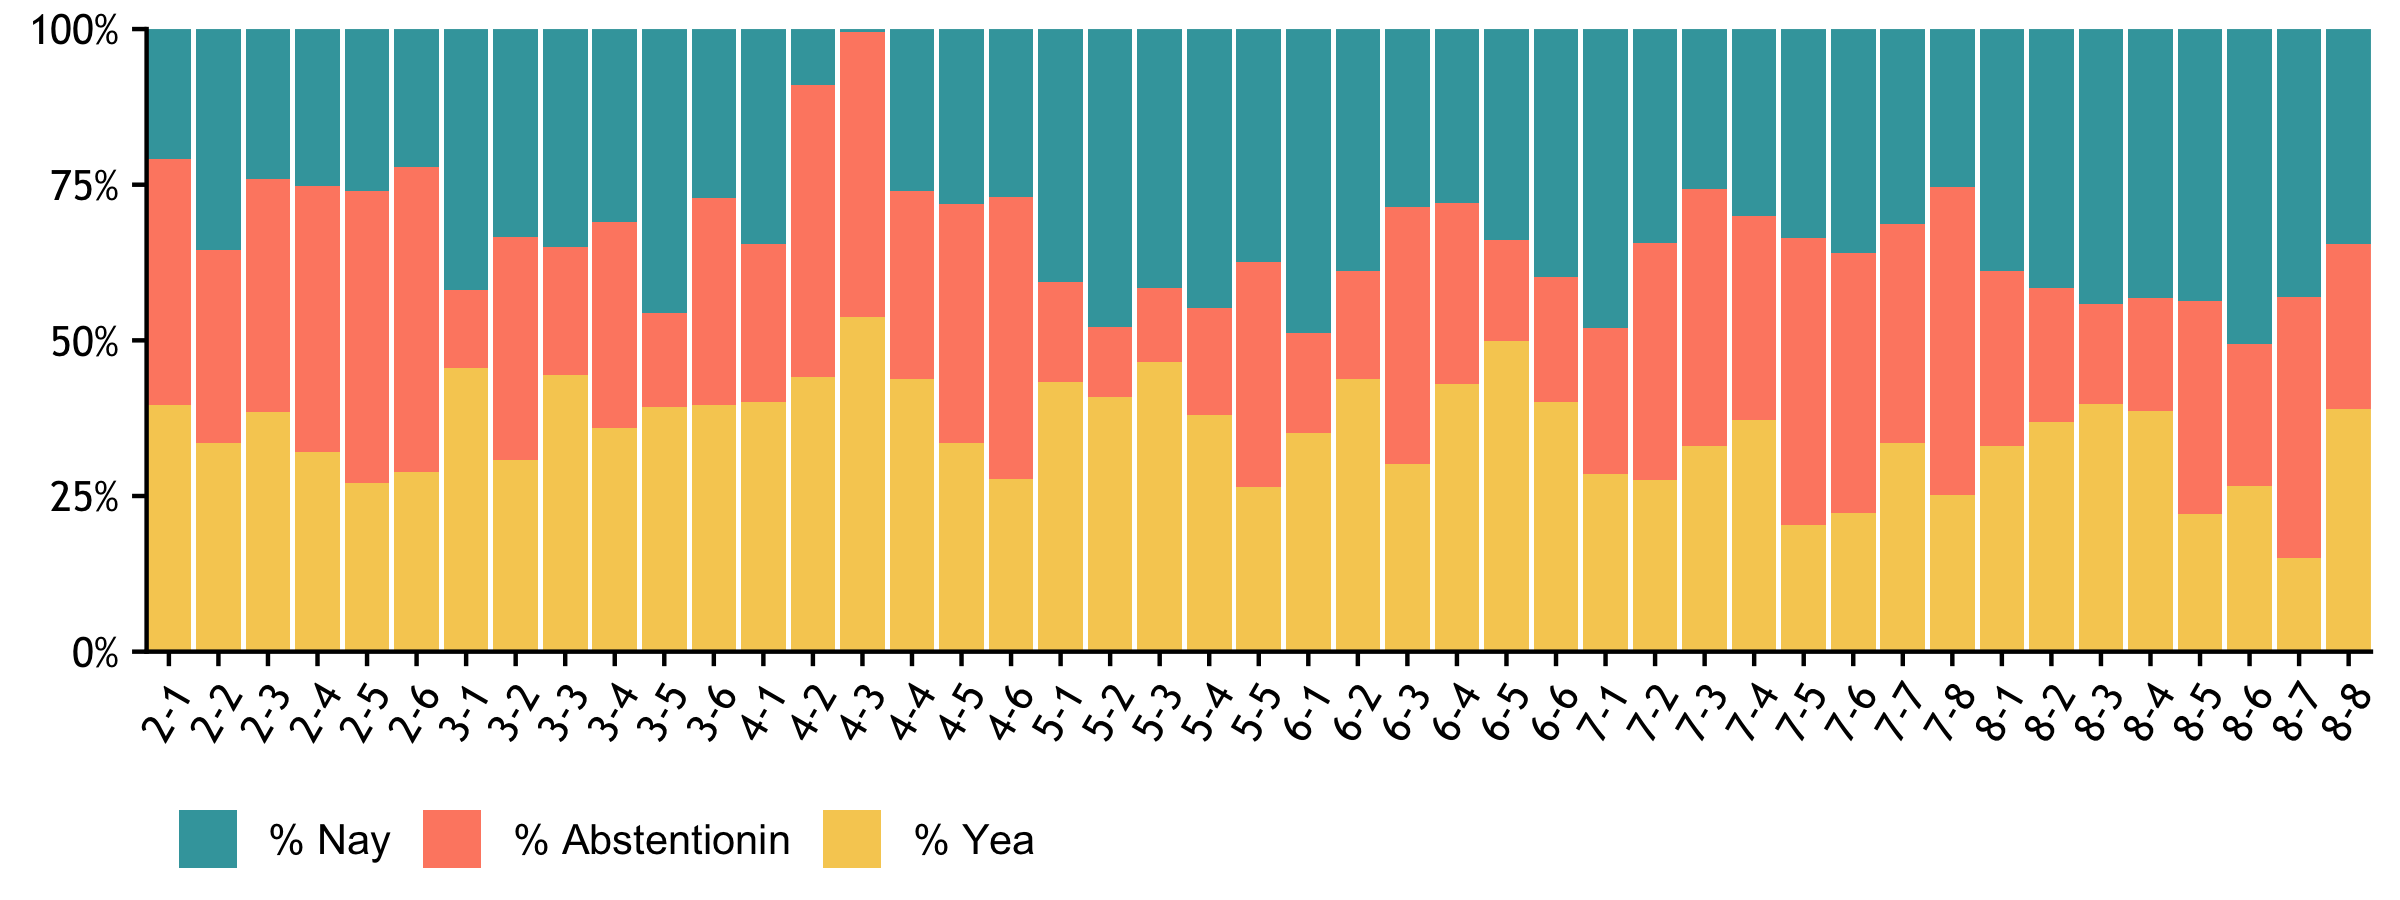
\includegraphics[width=14cm, height=6.8cm]{02-Chapter-Two/image/mean_rollcall.png}
    \caption{Proportions of Yea, Abstain  and Nay Votes \\ across Sessions}
    \label{fig:vote-distribution}
\end{figure}


\section*{\centering The Measurement of Legislator' Positions}


The spatial model of binary choice have revealed numerous insights into the structure and dynamics of legislative voting \citep[][]{Carroll2013,Clinton2004,Cox2002b, McCarty2001,McCarty2006,Snyder2001,Poole1997,Poole2007,Jackman2001,Tsai2020,Gray2019} and judicial preferences \citep[][]{Epstein2007,Martin2002,Martin2007}. In recent years, Item Response Theory based measure of legislative voting developed by \textcite{Clinton2004} has been successful in its application to understand legislative voting \citep[e.g.][]{Zucco2011, Tsai2020, Gray2019}. In its application, legislators as subjects possess a latent level of ability measured by varieties of roll calls and political ideology as ability. The IRT measure can be utilised to set up item difficulty parameters to discover estimates of the voting preferences of legislators.

In particular, I estimate a separate ideological position for each legislator at the frequency of session. The parameters for bills are assumed to be fixed across legislative sessions, so that I can estimate the positions of legislators over time. There are $N$ unique legislators who voted bills and they are indexed by $i$, i.e. $i=1,2,...,N$. Let $J_{t}$ denote the total number of bills voted in the $t$th session, where $t$ does not exceed the total number of sessions, 40. For simplicity, denoted $j$ by the $j$th bill voted in the session $t$, where $j\leq J_{t}$. $i$ and $j$ record the location of the data in the dimension of legislators and bills, respectively. Therefore, the ``nay'' or ``yea'' vote by legislator $i$ for the $j$th bill in the session $t$ is denoted by $y_{ijt}$. If ``nay'' vote is recorded, $y_{ijt}=0$, and if ``yea'' vote is recorded, $y_{ijt}=1$. 

Given these notations, I can proceed to apply the Expectation-Maximisation (EM) algorithm introduced by \citet{Imai2016} to estimate the dynamic ideal point model with binary outcomes. First, the single-dimension ideal point model is specified by

\begin{equation}
\begin{aligned}
Pr(y_{ijt}=1)=\Phi(\alpha_{jt}+\beta_{jt}x_{it})=\Phi(\tilde{x}_{it}\tilde{\beta}_{jt}^{T}),
\end{aligned}
\end{equation}

\noindent where $x_{it}$ is the $i$th legislator's ideal point at time session $t$, and $\alpha_{jt}$ and $\beta_{jt}$ represent the item difficulty and item discrimination parameters for the bill $j$ at session $t$. The second half of the equation expresses it into the vector form, where $\tilde{x}_{it}=(1,x_{it})$ and $\tilde{\beta}_{jt}=(\alpha_{jt},\beta_{jt})$. Further, the latent propensity $y_{ijt}^{*}$ is introduced, such that 

\begin{equation}
\begin{aligned}
{y_{ijt}^{*}=\tilde{x}_{it}\tilde{\beta}_{jt}^{T}+\zeta_{ijt},}
\end{aligned}
\end{equation}


\noindent where $\zeta_{ijt}\sim N(0,1)$ are $i.i.d$ shocks. The legislator $i$ ideal point process is specified through the following conditional (on prior) distribution:

\begin{equation}
\begin{aligned}
{x_{it}|x_{it-1}\sim N(x_{it-1},\sigma_{x}^{2}),}\label{eq:ideal-point}
\end{aligned}
\end{equation}

\noindent for $t=1,2,3,...,40$. In addition, I assume the initial prior for $t$ = 1 to be $x_{i0}\sim N(\mu,\Sigma_{x})$ for each legislator and choose the KMT party whip as the anchor subject. Note that different sets of legislators participated in different legislative sessions and in each session, different set of bills were voted. For legislators who abstained or were not in legislature at session $t-1$, the average ideological point within their party at session $t-1$, $\tilde{x}_{it}$, is used as their prior at session $t$. Ideological estimates are robust to different methods of generating missing priors.\footnote{For the estimation of ideal points, I use the \textbf{biIRT()} function from the \textbf{emIRT} package \citep[see][]{emIRT2021}. This function estimates a binary IRT model with two response categories, Yea and Nay. Subsequently, I use \textbf{makePriors()} function to generates diffuse priors as several matrices of starting values for the parameters, based on the number of legislators $N$, the number of bills $J$ and the number of a dimension $D$. That is, the parameters include prior means and covariance matrix for ideal points $x_{it}$ and $\alpha_{jt}$, $\beta_{jt}$, respectively. Note that the package currently supports estimation from one dimension, which means the number of the dimension $D$ is 1 (a single dimension). As for item difficulty $\alpha_{jt}$, item discrimination $\beta_{jt}$ and legislators' ideal points $x_{it}$, I use \textbf{getStarts()} function to generate the matrices of the parameters for first session.} 

Joint posterior distribution set up in this paper  is same as the equation (31) from \citet{Imai2016}. The estimation is conducted using the EM algorithms which consists of three steps as is described by equation (60)-(64) in their paper and discussed in \citet{Armstrong2020}. Moreover, \citet{Imai2016} found that the algorithm yields similar and comparable ideological estimates to the standard Markov chain Monte Carlo algorithm, but will process much faster and better with massive data. In this paper, I examine the impact of electoral reform in 2008 on within- and between-parties ideological dispersion. In fact, by using this model, where legislators form ideal points based on a Bayesian approach (process \autoref{eq:ideal-point}), I leave large room for inter-dependence and autocorrelation between ideal points. Later I show, despite of this setting, the occurrence of the electoral reform generates increased gaps between inter-party division and intraparty distance at the individual level. 

\subsection*{Ideal Point of Estimated Individual Legislators}

\autoref{fig:year-plot} plots estimated distributions of individual legislator's ideological positions clustered by parties for the two major parties (KMT and DPP) at a frequency of year from 1996 to 2015.\footnote{Appendix \ref{sec:Plots full} shows the estimated distributions for both parties at a frequency of session and all minority party a frequency of year. The top shaded area displays post-reform distributions and the bottom area illustrates pre-reform distributions of ideological positions.} Several patterns are illustrated from the figure. First, the distributions of DPP and KMT legislators' ideological positions started to shift to both poles when the reform occurred (year 2008), meaning that there was a drastic divergence in ideological positions between DPP and KMT legislators. This can be interpreted as a piece of evidence of inter-party political polarisation between DPP and KMT.\footnote{\autoref{fig:individual_point} in Appendix \autoref{sec:Plots full} shows individual legislator's positions grouped by year for both major parties (DPP and KMT).} Second, the distribution of ideological positions, particularly KMT, started to spread out across the spectrum after the reform, indicating that the intraparty ideological dispersion is exacerbated after the reform. Note that DPP tends to be ideologically cohesive across year, while KMT tend to be much more disperse, particularly in 2008 to 2010. This suggests that despite the unification of co-partisan legislators' position, different parties are witnessed to polarise their positions along the ideology spectrum. Moreover, the SMD demonstrates heterogeneous effects on two major parties. DPP become less polarised and its average ideology is neutralised, while KMT witnesses a further intraparty divergence in ideology, spreading across both ends of the spectrum.

\begin{figure}[ht]
\caption{Estimated Legislators' Ideological Positions for Major
Parties, Grouped by Party and Year \label{fig:year-plot}
}\centering{}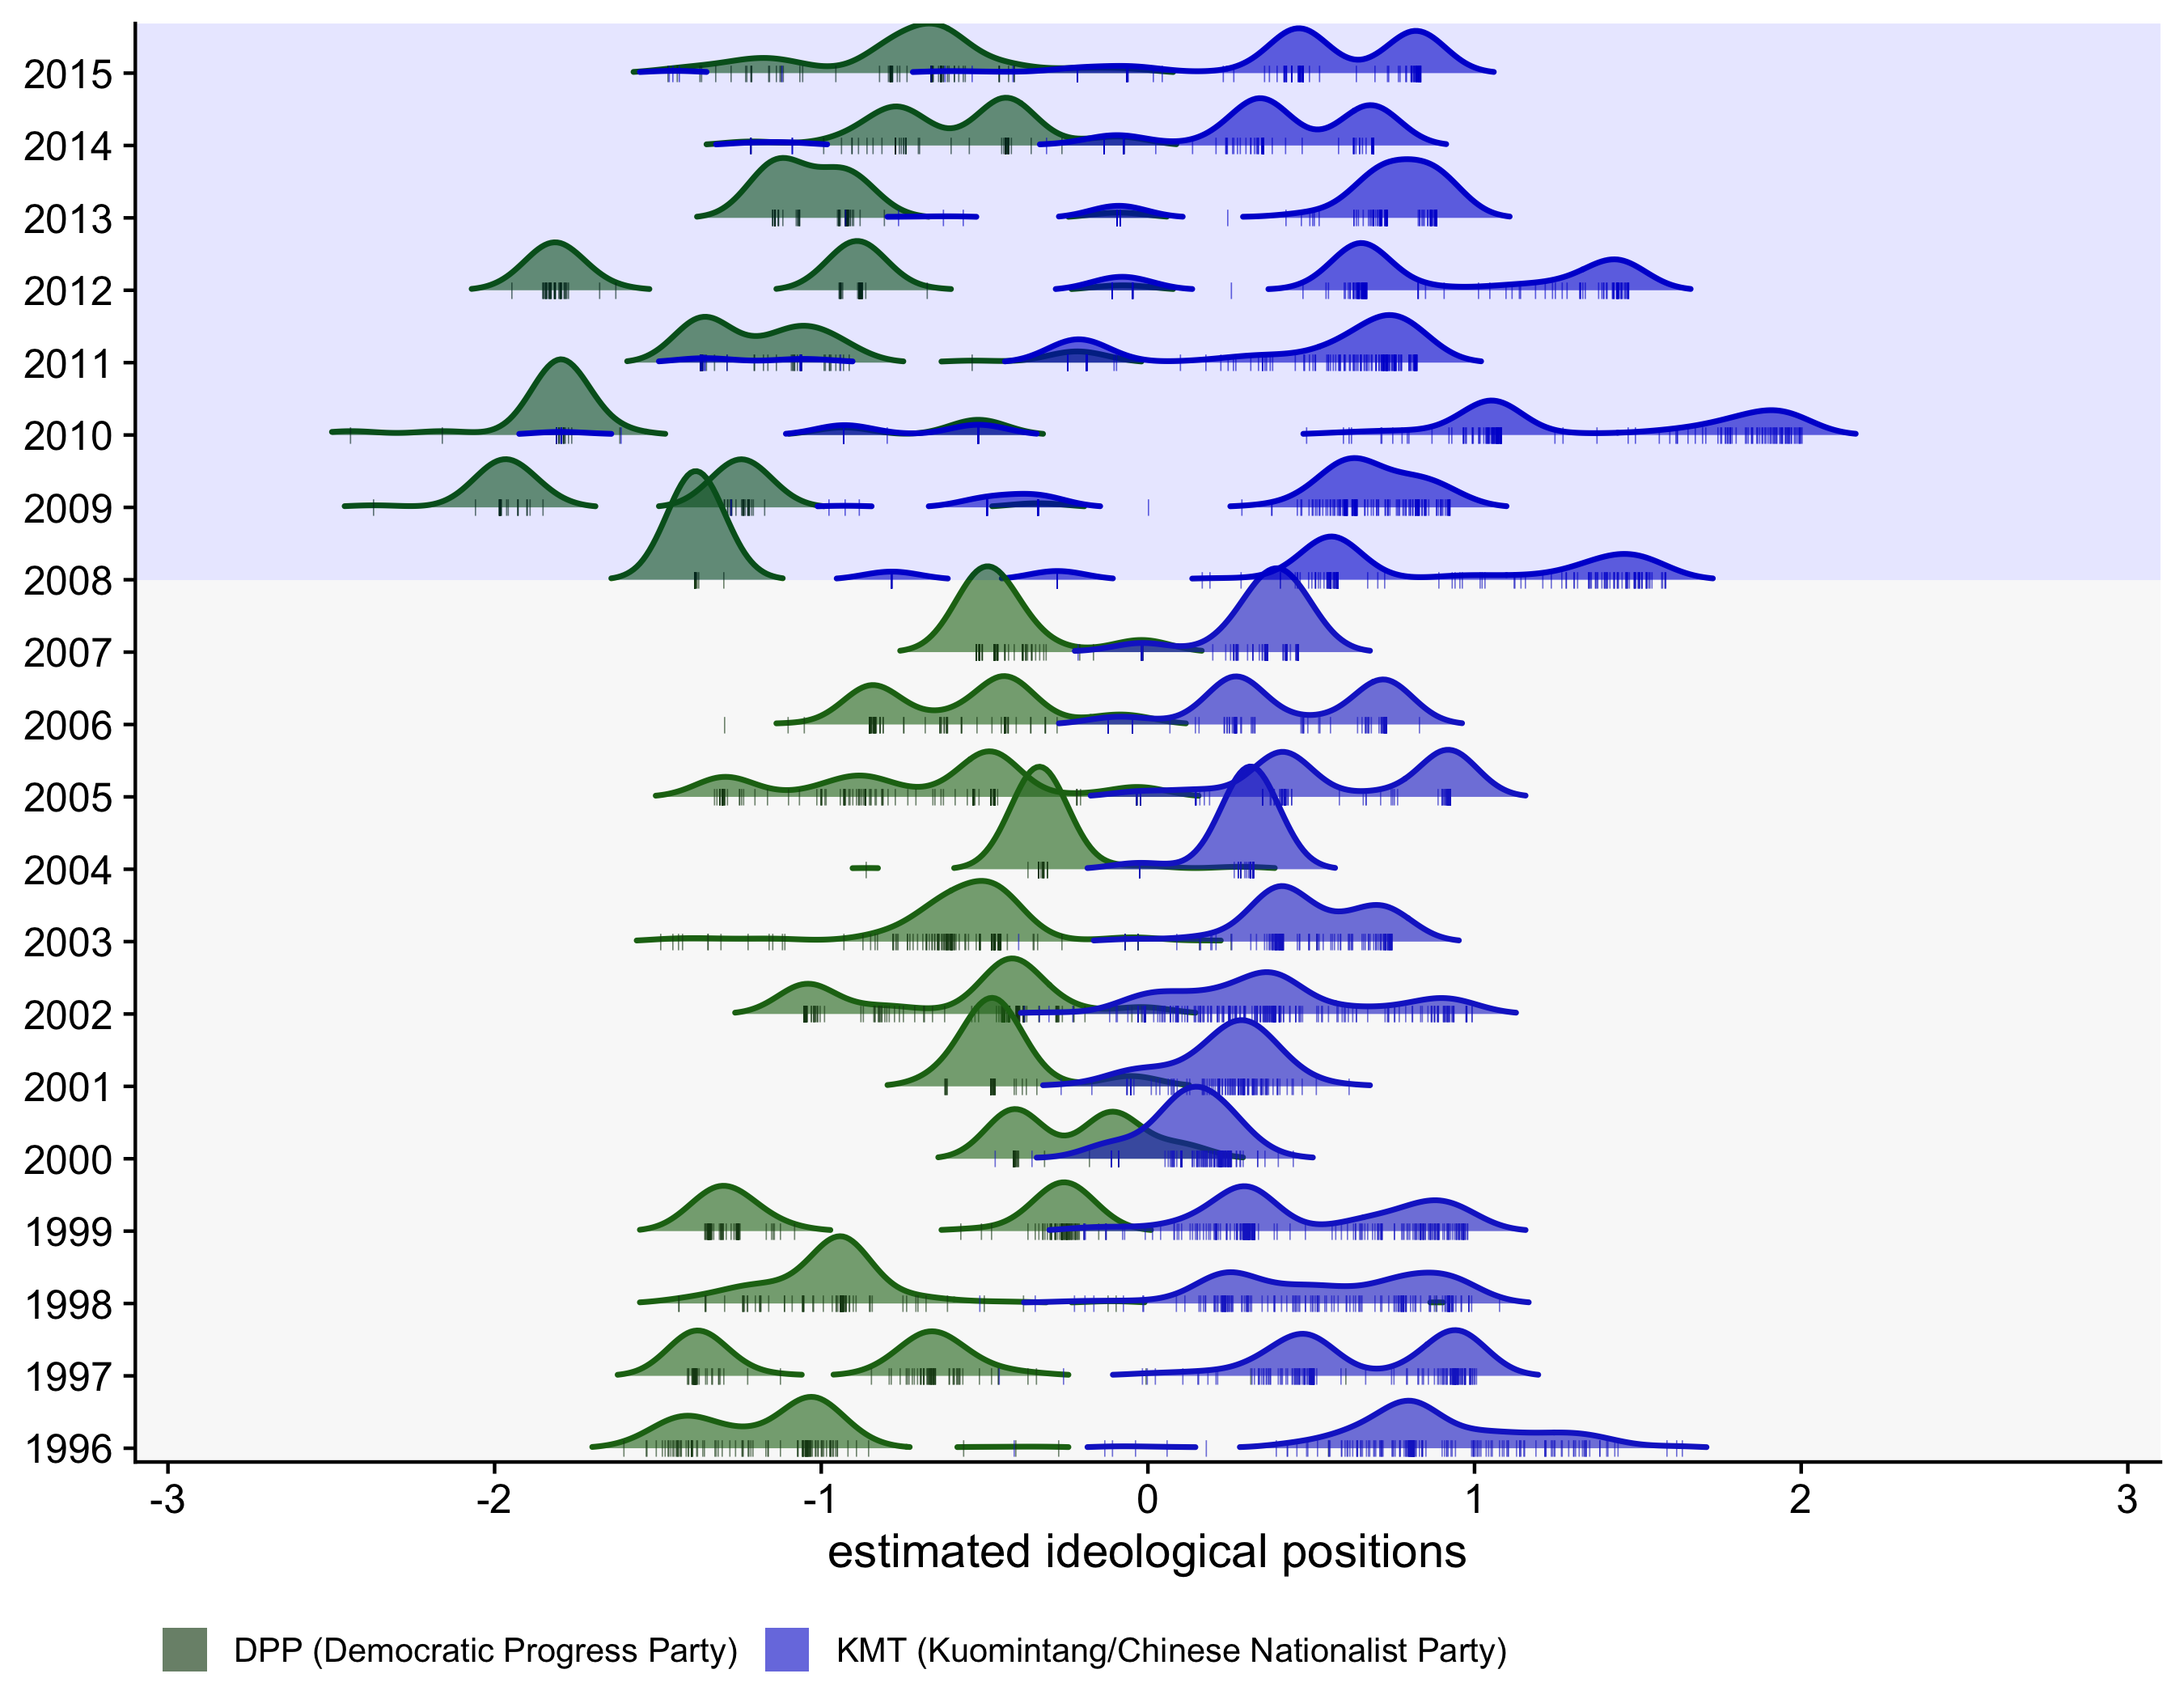
\includegraphics[scale=0.15]{02-Chapter-Two/image/major_postions_year.png}
\end{figure}

\subsection*{Party and Party Whip}

\begin{figure}[ht]
    \centering{}\caption{\label{Fig:2-1}
    Estimated Party Average and Party Whip's of Positions across Sessions \label{fig:whip_mean}}
    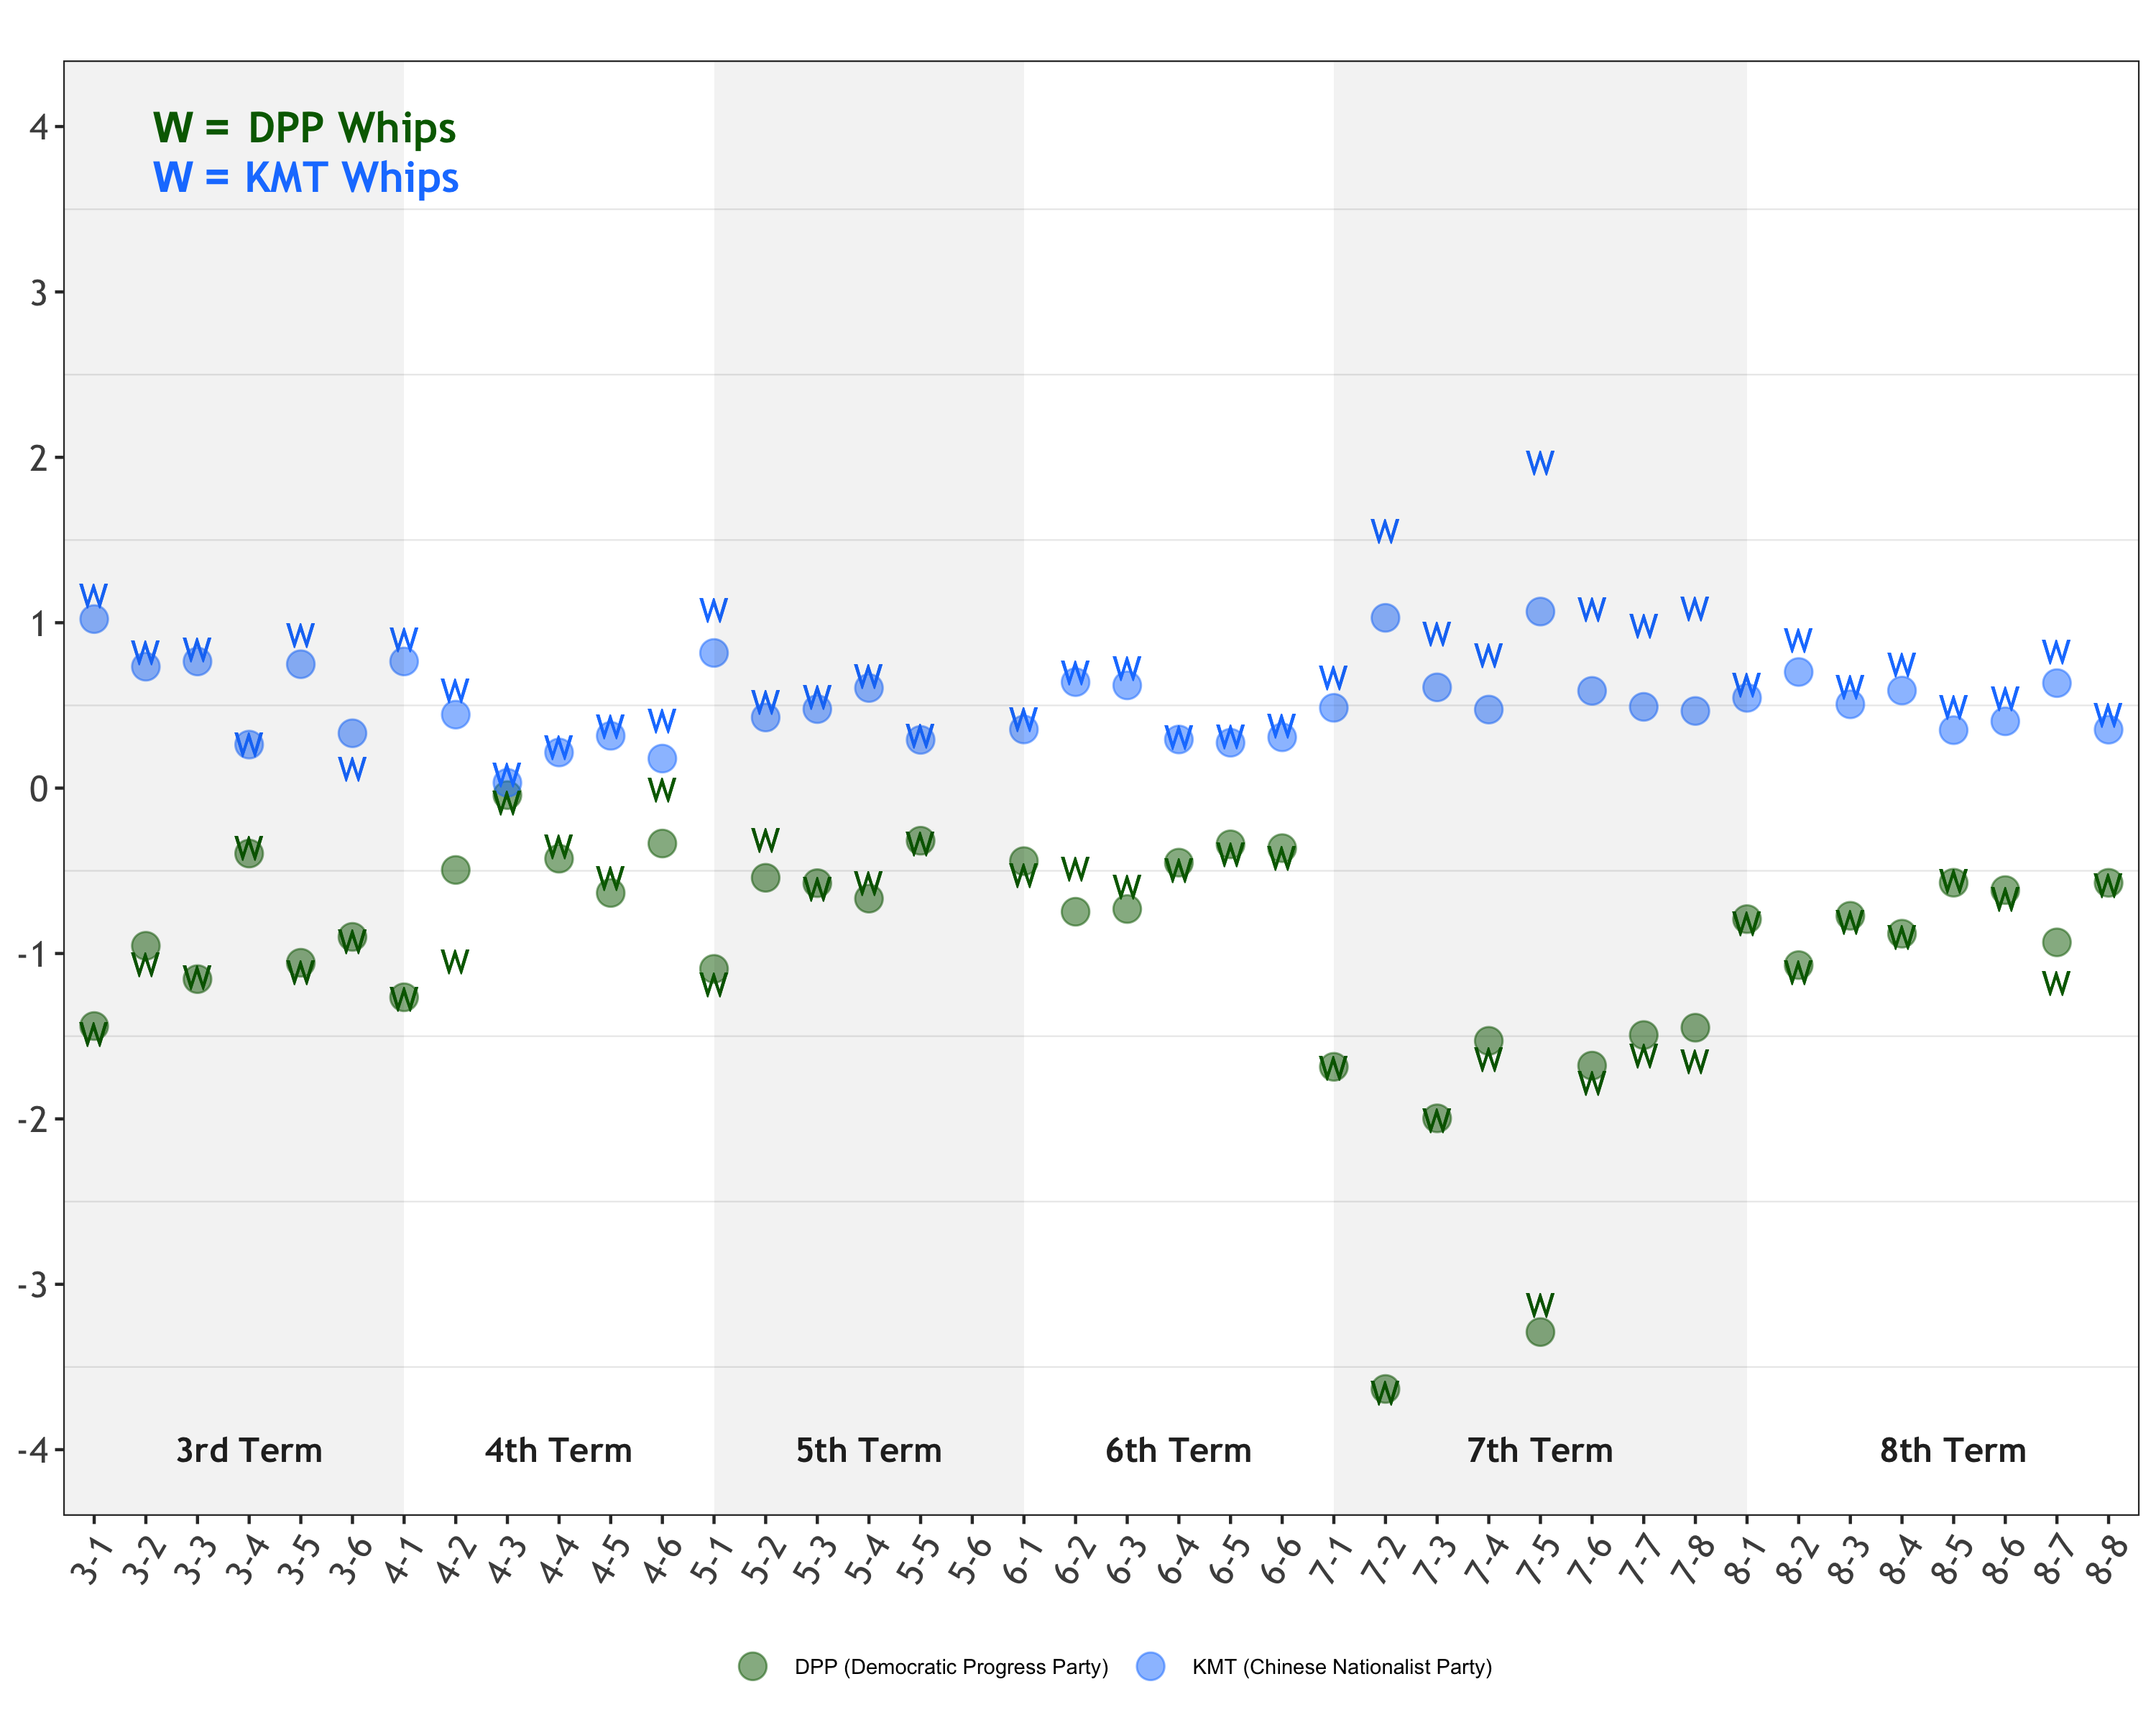
\includegraphics[width=14cm,height=9.5cm]{02-Chapter-Two/image/partywhip_mean}
\end{figure}

\autoref{fig:whip_mean} plots the estimated the average of party position and party whip's positions against sessions.\footnote{For KMT and DPP party whip's ideological positions are used to measure representative party positions, while for minor parties the average party ideological positions are used to measure representative party positions. This is due to the fact that in some sessions, party whips from some minor parties are not elected as legislators.} The figure displays the average estimated positions in each of the two major parties, KMT (denoted by ``blue dots'') and DPP (denoted by ``green dots''), while \textbf{\textit{W}} labels the party whip's positions for each party.\footnote{Apart from KMT and DPP, legislators from other minor parties are also included in the observation and used for regressions in column 1 and 2 in \autoref{tab:intra-estimation}.} \autoref{tab:Correlation} summarises some correlation statistics of the two major parties, DPP and KMT, showing that party average and party whip's ideological positions in the same party share a similar pattern (positive high correlation), while party average (or party whip's) ideological positions between KMT and DPP move in a quite opposite direction (negative high correlation). This implies the existence of political polarisation in terms roll call votes between KMT and DPP, and they are considered as rival parties.\footnote{Party whip plays an important role to ensure their co-partisans to vote policy position according to instructions made by their party central committee, rather than the will of their constituents. When voting for crucial bills or budget items, the whips may issue ``top-mobilisation order'' asking their legislators to attend voting sessions. Legislators disobeying the orders from party whips may be fined, suspended or even expelled from the party \citep{Hsu2002}.} 

Moreover, I specifically test in each party, if the average party voting behaviour seamlessly obeys the party's voting instruction (the whip's behaviour) across time using the following regression

\begin{equation}
whip_{it}=c_{i}+\phi_{i}\bar{party_{it}}+\zeta_{it}^{0},
\end{equation}

\noindent where $whip_{it}$ is the party $i$ whip's position, $\bar{party_{it}}$ is the corresponding party's average ideological position at session $t$, and $c_{i}$ is a constant. If the the average party voting behaviour follows the whip's voting behaviour, i.e. the the average obeys the party's instruction, constant $c_{i}=0$ and the coefficient $\phi_{i}=1$, simultaneously.

\begin{table}[ht]
\caption{Correlation Statistics of Estimated Position for Major Parties\label{tab:Correlation}}
\begin{centering}
\begin{tabular}{|c|cccc|}
\hline 
    \textbf{Correlation}                                & 
        $\overline{\textbf{party}}_{\textbf{KMT}}$          & 
        $\overline{\textbf{party}}_{\textbf{DPP}}$          &
        $\textbf{whip}\mathbf{_{KMT}}$                      &
        $\textbf{whip}\mathbf{_{DPP}}$                    \\
    \hline 
        $\overline{\textbf{party}}_{\textbf{KMT}}$          & 
        \done 1                                             &  
                                                            &  
                                                            & 
                                                            \tabularnewline
        $\overline{\textbf{party}}_{\textbf{DPP}}$          & 
        -0.702                                              & 
        \done 1                                             &
                                                            &
                                                            \tabularnewline
        {$\textbf{whip}\mathbf{_{KMT}}$}                    & 
         0.874                                              & 
        -0.881                                              & 
        \done 1                                             & 
                                                            \tabularnewline
        $\textbf{whip}\mathbf{_{DPP}}$                      & 
        -0.688                                              & 
        0.987                                               & 
        -0.870                                              & 
        \done 1                                             \tabularnewline
\hline 
\multicolumn{5}{l}{{$\overline{party}_\mathbf{i}$ denotes the average
position for party $i$, and $\mathbf{whip_{i}}$ }}         \tabularnewline
\multicolumn{5}{l}{{denotes the whip's position for party$i$, $i=KMT$ or $DPP$.}}                                                                         \tabularnewline
\end{tabular}
\par\end{centering}
\end{table}


Panel A in \autoref{tab:whip-position} reports regression outcomes for two major parties, individually. Panel B shows testing results using F test. As is illustrated in Panel B, I fail to reject the null of obedience to party instruction for DPP, while I reject the null for KMT, indicating the average DPP party voting behaviour seamlessly obeys whip's behaviour and KMT otherwise. Moreover, above test outcomes also justify when proceeding to test \textbf{Hypotheses \ref{h:p1-h1}} and \textbf{\ref{h:p1-h2}} respectively, I calculate inter- and intraparty ideological dispersion for both KMT and DPP respectively using the ideological differences between individual legislators and the corresponding party whip, due to this discrepancy in whip's position and average party position.


\begin{table}[tp]
\caption{Testing for the Obedience of Legislators' Voting Behavior
to Instruction Issued by Party Whip
\label{tab:whip-position}}

\centering{}%
\begin{tabular}{lcc}
\toprule 
 & \textbf{DPP} & \textbf{KMT}\tabularnewline
\midrule 
\multicolumn{3}{l}{\textbf{Panel A: regression results}}\tabularnewline
\multicolumn{3}{l}{\textbf{Dependent variable: }whip's position}\tabularnewline
\midrule 

\textbf{average party position} & {1.000$^{***}$} & {1.304$^{***}$}\tabularnewline
 & (0.027) & (0.119)\tabularnewline
\textbf{constant} & -0.023 & 0.023\tabularnewline
 & (0.033) & (0.068)\tabularnewline
\textbf{No. of observations} & 39 & 39\tabularnewline
\textbf{Adjusted \textit{R}$^{2}$} & 0.97 & 0.76\tabularnewline
\textbf{Prob > F} & 0.00 & 0.00\tabularnewline
\midrule
\multicolumn{3}{l}{\textbf{Panel B: testing outcomes}}\tabularnewline
\midrule
\multicolumn{3}{l}{\textbf{$\mathbf{H_{0}}$}:\textbf{ $c_{i}=0$ }and\textbf{ $\phi_{i}=1$}}\tabularnewline
\textbf{Prob > F} & 0.307 & 0.000\tabularnewline
\textbf{Reject $H_{0}$} & No & Yes\tabularnewline
\midrule
\multicolumn{3}{l}{{Asterisk indicates significant level: {*}: p < 0.10;
{*}{*}:}}\tabularnewline
\multicolumn{3}{l}{{p < 0.05; {*}{*}{*}:p < 0.01.}}\tabularnewline
\end{tabular}
\end{table}


\section*{\centering Empirical Findings}

I merge validated estimates of legislators' ideological positions across sessions with legislator profiles and election data from the database of the Taiwanese Legislative Yuan (Congress Research Services), and perform statistical tests below.

\subsection*{Interparty Polarisation\label{subsec:political-polarization}}

To evaluate the \textbf{Hypothesis \ref{h:p1-h1}}, I calculate the legislator-level inter-party dispersion between two major parties, KMT and DPP (between party polarisation). The inter-party dispersion is defined as the distance of ideological positions between individual legislator and the opponent party whip in each legislative session, \boldsymbol{$interdistance_{it}$}. It is calculated as: 

\begin{equation}
\mathbf{interdistance_{it}=|position_{it}-\bar{whip_{it}|}},
\end{equation}

\noindent where $position_{it}$ denotes the ideological position of legislator $i$ at session $t$ and $\bar{whip_{it}}$ denotes the ideological position of the opponent party whip for legislator $i$ at time $t$. For instance, if legislator $i$ is affiliated to KMT (DPP), then $interdistance_{it}$ is the ideological distance between his estimated position and DPP (KMT) whip's estimated position, at session $t$.

Following \citet{Catalinac2017}, I specify the following regression model, allowing the passage of time (year) to have different marginal effects on inter-party ideological distance, prior to and post the electoral reform.

\begin{align}
\mathbf{interdistance_{it}=\alpha_{0}+\alpha_{1}electoralreform_{t}+\alpha_{2}year_{t}+}\nonumber \\
\mathbf{\alpha_{3}(year_{t}\times electoralreform_{t})+C_{it}+\epsilon_{it}^{1},}\label{eq:interdistance}
\end{align}

\noindent where $year_{t}$ is the year dummy indicating in which year the session $t=1,2,...,39$ (pertaining the 1st, the 2nd, the 3rd,..., the 39th session in our observation, respectively) is held.\footnote{Total 39 sessions is due to the lack of data for the 5-6 session in year 2005.} $electoralreform_{t}$ is a dummy variable showing whether an observation belongs to the post-transition phase (i.e. if $t\geq24$) if $electoralreform_{t}=1$. $C_{it}$ contains controls pertaining to legislator $i$ and in session $t$: legislator attributes, party-affiliation dummies, and electoral district attributes. Specifically, legislator attributes include each legislator's sex and marginal winning share. Marginal winning share is defined as the excessive percentage points of votes the legislator won comparing to the legislator who won the next most votes. Party-affiliation dummy here is denoted by $KMT$. If the legislator $i$is affiliated to KMT, $KMT=1$; otherwise, $KMT=0$. Electoral district attributes control for the size of each electoral district: if a district's magnitude is over 9, $bigdistrict=1$ and $middistrict=0$; if its magnitude is between 5 to 8, $bigdistrict=0$ and $middistrict=1$; if its magnitude is below 5, $bigdistrict=0$ and $middistrict=0$. And the standard assumptions of homoskedasticity apply to the error term $\epsilon_{it}^{1}$.

\begin{table}[ht]
\caption{Interparty Ideological Differences\label{tab:inter-estimation}}

\centering{}%
\scalebox{0.95}{
\begin{tabular}{lcc}
\toprule 
\multicolumn{3}{l}{\textbf{Dependent variable:}}\tabularnewline
\multicolumn{3}{l}{Interparty Ideological Differences between Mainstream Parties}\tabularnewline
\midrule
 & \textbf{interaction} & \textbf{(+ controls)}\tabularnewline
\midrule
\textbf{electoral reform} & 16.21{9$^{***}$} & 15.291{$^{***}$}\tabularnewline
 & (0.747) & (0.867)\tabularnewline
\textbf{year} & {-0.242$^{***}$} & -0.238{$^{***}$}\tabularnewline
 & (0.008) & (0.010)\tabularnewline
\textbf{year }\textbf{$\times$ electoral reform} & -0.643{$^{***}$} & {-0.599$^{***}$}\tabularnewline
 & (0.040) & (0.046)\tabularnewline
\textbf{marginal winning shares} &  & 0.026\tabularnewline
 &  & (0.202)\tabularnewline
\textbf{intercept} & 3.40{5$^{***}$} & 3.697{$^{***}$}\tabularnewline
 & (0.071) & (0.252)\tabularnewline
\textbf{legislator attributes} &  & $\checkmark$\tabularnewline
\textbf{party dummies} &  & $\checkmark$\tabularnewline
\textbf{district fixed effects} &  & $\checkmark$\tabularnewline
\midrule
\textbf{No. of observations} & 5663 & 4170\tabularnewline
\textbf{Adjusted \textit{R}$^{2}$} & 0.28 & 0.27\tabularnewline
\textbf{Prob > F} & 0.00 & 0.00\tabularnewline
\midrule
\multicolumn{3}{l}{{Robust standard errors are reported in parentheses. Asterisk indicates}}\tabularnewline
\multicolumn{3}{l}{{significant level: {*}: p < 0.10;
{*}{*}: p < 0.05; {*}{*}{*}:p < 0.01.}}\tabularnewline
\end{tabular}}
\end{table}

\autoref{tab:inter-estimation} reports the estimation results, where the dependent variable is legislator's inter-party ideological distance. Both \textbf{electoral reform} and \textbf{year $\times$ electoral reform }are statistically significant, with (column 2) or without incorporating controls (column 1). Specifically, the coefficient on \textbf{electoral reform} is statistically significant (at 1\% critical level) in both cases, suggesting electoral reform had a significant positive impact on the inter-party ideological distance between the two major parties (KMT and DPP), even when the passage of time (year) and other legislator-, party- and district-level attributes are controlled for. After the reform, a typical legislators from KMT (DPP) underwent a phase of polarisation in terms of the roll call votes, i.e. her ideological positions became further away from the DPP (KMT). Therefore, the estimation rejects the \textbf{Hypothesis \ref{h:p1-h1}} and the electoral reform significantly polarised legislators from the rival party. \autoref{fig:inter-fitted} plots the fitted value of legislator-level inter-party ideological distance with their 95\% confidence intervals against year. At 2008 (when the reform occurred), there was a drastic leap in between-party ideological distance. The significance of the coefficient on the interaction term \textbf{year $\times$ electoral reform} implies that the passage of time (year) indeed had heterogeneous effect on between-party distance. It also shows that the increase in time resulted in lower-level distance.\footnote{To ensure these results are not driven by any individual major party, Appendix \ref{sec:robustness-check} reports the estimation results separately for the two major parties and verify the consistency and robustness of results.} 

\begin{figure}[ht]
\caption{Fitted Values of Inter-party Ideological Distance between KMT and DPP with 95\% Confidence Intervals \label{fig:inter-fitted}}\centering{}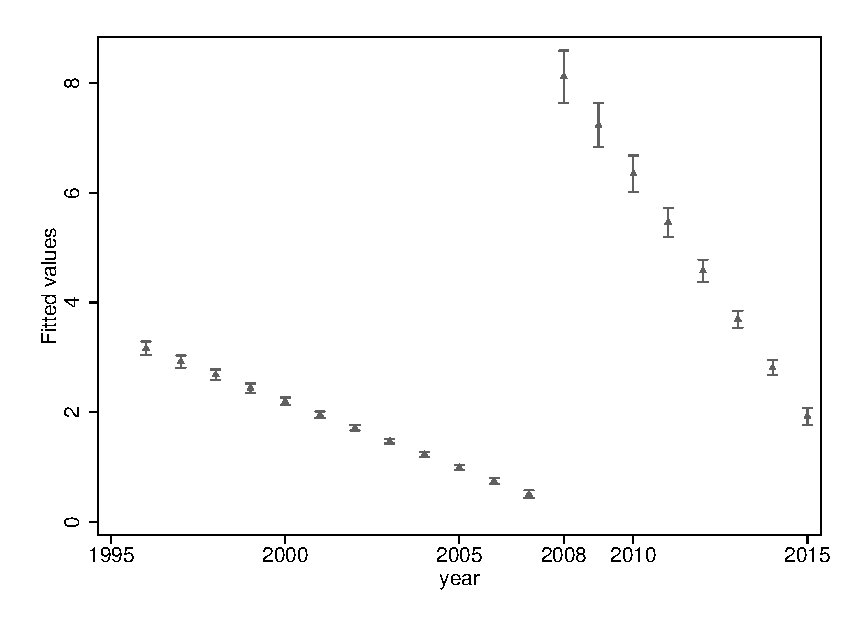
\includegraphics[scale=0.59]{02-Chapter-Two/image/all_inter.eps}
\end{figure}

\autoref{fig:individual_legislators} shows seven most senior legislators and individual legislators' ideal points for two major parties, KMT (denoted by ``K'') and DPP (denoted by ``D''). As illustrated in \autoref{fig:individual_legislators}, two major parties diverge drastically after the introduction of SMD in the 7th session. Note that the ideological positions of the seven most senior legislators, including five KMT and three DPP legislators, who have served in the Legislative Yuan over twenty years, are highlighted and aligned individually in the figure. It clearly demonstrates how the electoral reform in 2008 changes their positions: senior legislators from KMT and DPP tend to be more spatially converged under the SNTV system, whereas both parties appear to diverge against each other under the SMD, also consistent with our empirical findings.

\begin{figure}[ht]
\caption{Ideal Point of Individual Legislator \label{fig:individual_legislators}}\centering{}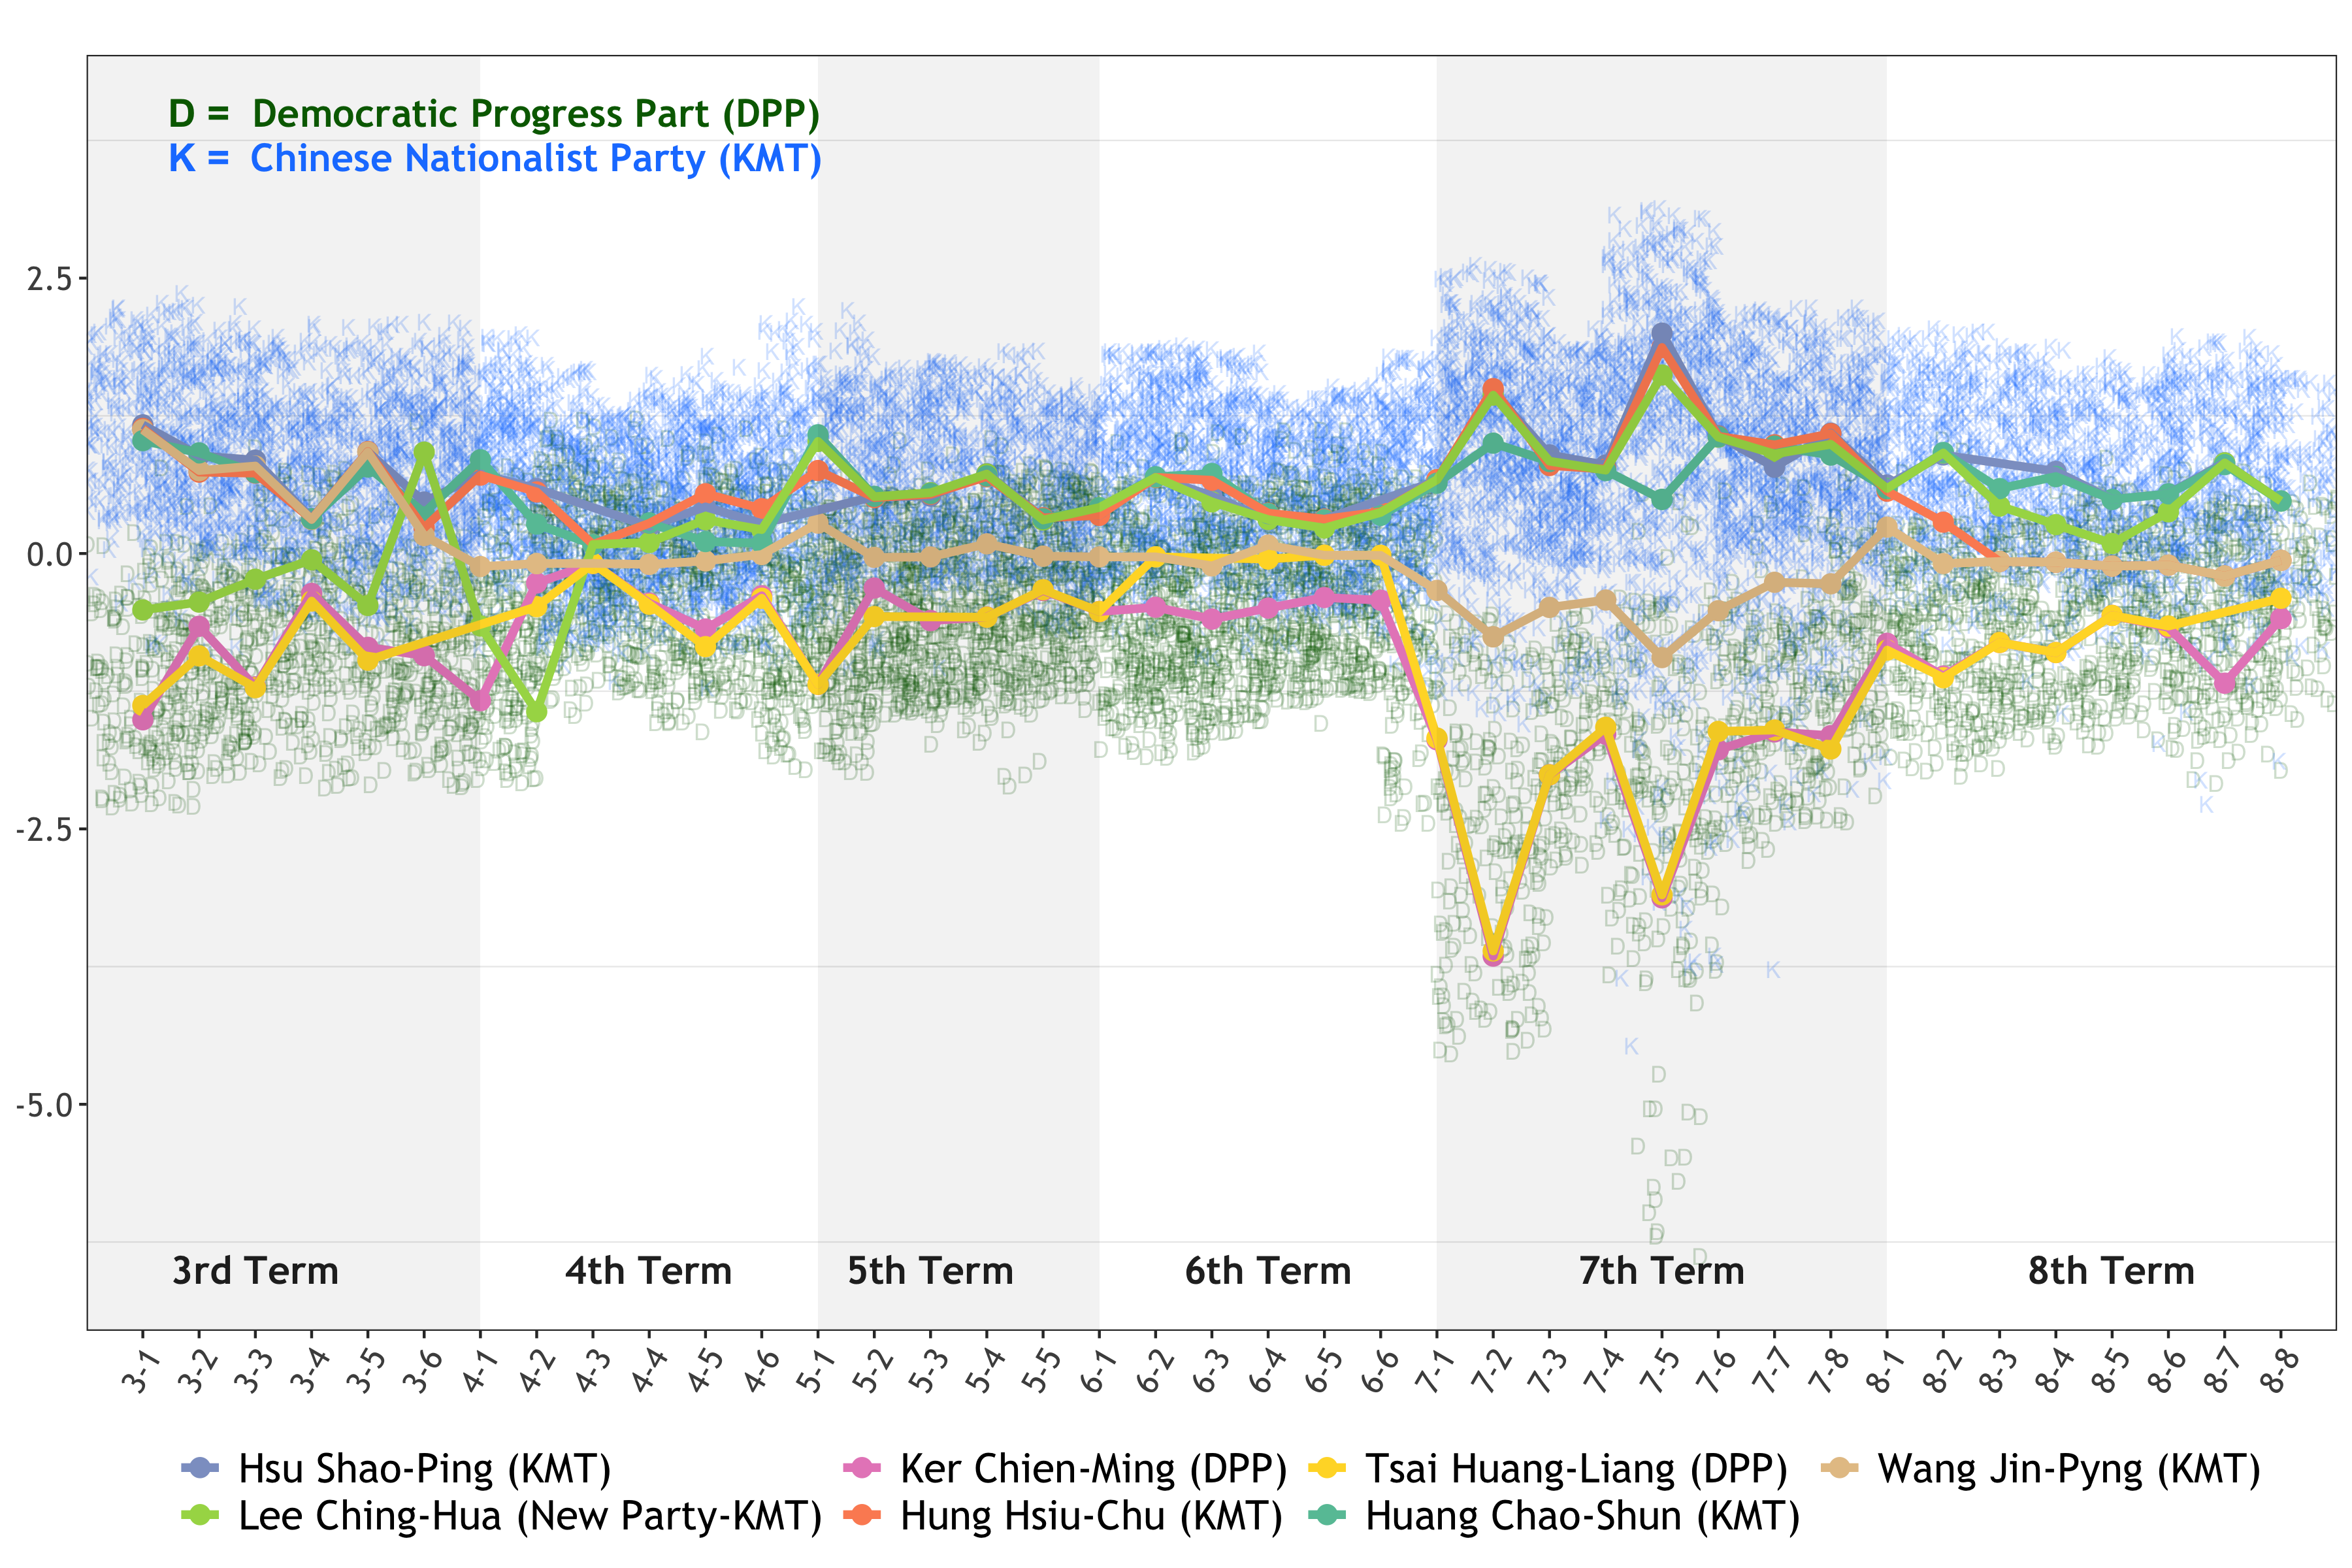
\includegraphics[width=13cm, height=9.5cm]{02-Chapter-Two/image/seven_legis}
\end{figure}

\citet{Catalinac2017} illustrates the robustness using sub-sample only including competitive candidates. In our regression, I include \textbf{marginal winning share} of each legislator in each legislative session as a control, which implies the competitiveness of the corresponding legislator. As it is not statistically significant (p > 0.10), it suggests that our estimation results are robust to using competitive legislators as the sample. Also, some are concerned that the inter-party dispersion were caused by the heterogeneity in bills voted across time, i.e. in some years, controversial bills (which are more likely to cause inter-party dispersion) are voted. To show that the inter-party dispersion before and after the reform was not caused by such heterogeneity, Appendix \ref{sec:robustness-check} addresses this problem by controlling for as many year dummies as possible and finds the robustness of our results.


\subsection*{Disunity in Co-partisan Legislators after the Reform\label{subsec:disunity-in-co-partisan}}

To evaluate \textbf{the Hypothesis \ref{h:p1-h2}}, I calculate the dispersion in co-partisan legislator's estimated ideological positions (within-party disunity). The dispersion here is defined as the distance between individual legislator's ideological positions and the co-partisan whip in each legislative session, $intradistance_{it}$. It is calculated as: 

\begin{equation}
\mathbf{intradistance_{it}=|position_{it}-whip_{it}|,}
\end{equation}

\noindent where $position_{it}$ denotes the ideological position of legislator $i$ at session $t$ and $whip_{it}$ denotes the ideological position of the party whip for legislator $i$ at session $t$. The regression model is constructed as follow.

\begin{align}
\mathbf{intradistance_{it}=\beta_{0}+\beta_{1}electoralreform_{t}+\beta_{2}year_{t}+ \nonumber } \\
\mathbf{\beta_{3}(year_{t}\times electoralreform_{t})+\tilde{C}_{it}+\epsilon_{it}^{2},\label{eq:intradistance}}
\end{align}

\noindent where $\tilde{C}_{it}$ contains controls. The only difference between $C_{it}$ in model (\autoref{eq:interdistance}) and $\tilde{C}_{it}$ is that more party-affiliation dummies are included in the controls. The rest estimation strategy are same as previously defined in the model (\autoref{eq:interdistance}).

\begin{table}[h]
\caption{Intraparty Distance at the Sessional Level\label{tab:intra-estimation}}
\centering{}%
\scalebox{0.85}{
\begin{tabular}{lccccc}
\toprule 
\multicolumn{6}{l}{\textbf{Dependent variable:} } \\
\multicolumn{6}{l}{Intraparty Ideological Distances} \\
\midrule 
                                                 & 
        \multicolumn{2}{c}{\textbf{All parties}} &  
                                                 & 
        \multicolumn{2}{c}{\textbf{Major parties}} \tabularnewline
        \cmidrule{2-3} \cmidrule{5-6}
                                                 & 
        \textbf{interaction}                     & 
        \textbf{(+ controls)}                    &  
                                                 & 
        \textbf{interaction}                     & 
        \textbf{(+ controls)}                       \tabularnewline
\midrule

\textbf{electoral reform}   & 1.79{1$^{***}$}   & 2.375{$^{***}$}   &          & {1.823$^{***}$} & {2.464$^{***}$}  \\
                            & (0.255)           & (0.336)           &          & (0.263)         & (0.199)          \\
\textbf{year}               & -0.0{04$^{***}$}  & -0.0{03$^{**}$}   &          & -0{.003$^{***}$}& {-0.004$^{**}$}  \\
                            & (0.001)           & (0.002)           &          & (0.001)         & (0.002)          \\
\textbf{year$\times$ electoral reform}  & -0.{082$^{***}$} & {-0.114$^{***}$} &         & {-0.083$^{***}$} & -0.11{7$^{***}$} \\
                                        & (0.013)          & (0.017)          &         & (0.013)          & (0.018)\\
\textbf{marginal winning shares}        &                  & -0.121           &         &                  & 0.041\\
                                        &                  & (0.269)          &         &                  & (0.084)\\
\textbf{intercept}                      & 0.0{80$^{***}$}  & -0.125{$^{*}$}   &         & 0.07{8$^{***}$} & -0.142{$^{*}$}\\
                                        & (0.006)          & (0.073)          &         & (0.009)         & (0.083)\\
\textbf{legislator attributes}          &                  & $\checkmark$     &         &                 & $\checkmark$\\
\textbf{party dummies}                  &                  & $\checkmark$     &         &                 & $\checkmark$\\
\textbf{district fixed effects}         &                  & $\checkmark$     &         &                 & $\checkmark$\\
\midrule
\textbf{No. of observations}            & 6736             & 4969             &         & 5663            & 4170\\
\textbf{Adjusted R$^{2}$}               & 0.04             & 0.05             &         & 0.04            & 0.05\\
\textbf{Prob > F} & 0.00 & 0.00 &  & 0.00 & 0.00\\
\midrule
\multicolumn{6}{l}{{Robust standard errors are reported in parentheses. Asterisk indicates significant }}\tabularnewline
\multicolumn{6}{l}{{level: {*}: p < 0.10;
{*}{*}: p < 0.05; {*}{*}{*}:p < 0.01.}}\tabularnewline
\end{tabular}}
\end{table}

\autoref{tab:intra-estimation} reports the estimation results, where the dependent variable is legislator's within-party ideological
distance. Column 1 and 2 illustrate outcomes using observations from all parties with or without controls. The variable of \textbf{electoral reform} had
statistically significant positive (at 1\% critical level) impact on co-partisan ideological distance, even when I control for the passage
of time (year) and other legislator, party, and district attributes. After the reform, legislators became more distant from co-partisan
whips (i.e. more disunited) in terms of ideological positions. Therefore, I reject the \textbf{Hypothesis \ref{h:p1-h2}} and the electoral reform significantly dis-united co-partisan legislators. Although this finding is contrary to manifesto studies like \citet{Catalinac2017} that candidates position themselves more cohesively with other co-partisan candidates in single-member districts, it is generally complementary with study of \citet{Jang2019}'s seminar work on Taiwan legislative roll call of the entire period of the SNTV-MMD system, which argues that legislators have varying degree of personal vote incentives when they face different electoral challenges. 

\begin{figure}[ht]
\caption{Fitted Values of Intraparty Ideological Distances in 95\% Confidence Intervals \label{fig:intra-fitted}}
\centering{}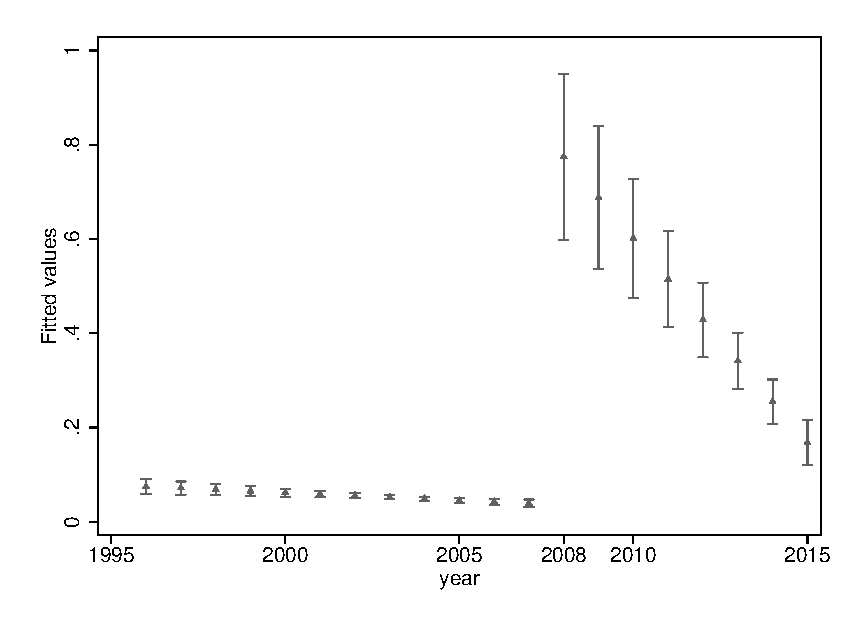
\includegraphics[scale=0.59]{02-Chapter-Two/image/KD_intra}
\end{figure}

The left-hand side in \autoref{fig:intra-fitted} plots the fitted value of intraparty ideological distance with their 95\% confidence intervals against year using the sample of legislators form all parties. At the 2008 (when the reform occurred), there was a leap in within-party ideological distance. Since the intersection term \textbf{year $\times$ electoral reform }is significant, time had heterogeneous effect on co-partisan ideological distance, before and after the reform. The outcomes also suggest that the increase in time was accompanies by lower levels of within-party distance. Column 3 and 4 show that the estimation is robust to using different sample of legislators (from the two major parties, KMT and DPP), with or without controls, respectively. The fitted value for this estimation is plotted at right-hand side in \autoref{fig:intra-fitted}. Moreover, since the control variable \textbf{marginal winning shares }is statistically insignificant, regression outcomes are also robust to use competitive legislators as the sample. To ensure these results are not driven by any individual major party, Appendix \ref{subsec:disunity-robust} reports the estimation results separately for the two major parties and finds the robustness of the results.

\section*{\centering Conclusion and Discussion}

This paper looks at a long-lasting myth of the impact of 2008 Taiwan electoral reforms. Although Taiwan transformed from SNTV to SMD, as scholars argue, some evidence indicates that SMD may not be as effective as originally thought in solving drawbacks of SNTV, such as polarized parties. Recently, conflicts between the two major parties
intensify and with-in party relationship becomes growingly rigid and tense. This project is a pioneer in empirically and formally testing the polarization and conflicts in legislator's attitude, prior and post the election reform using individual-level ideological positions extrapolated from legislative roll calls, adding contribution to a deeper understanding of potential impact of the reform on partisan relationship. 

Particularly, two hypotheses regarding the legislators' ideological positions are tested:1) switching from SNTV to SMD mitigated the level of political polarization between parties, particularly between
KMT and DPP; 2) switching from SNTV to SMD united co-partisan legislators in terms of ideological positions. Our findings suggest a phase of ``disunited polarization'' among inter-party and co-partisan legislators during the transition. Empirical test results show that the reform not only exacerbated inter-party ideological polarisation by distancing legislators' positions from their opponents, but also disunited co-partisan legislators as their positions became more widely distributed along the ideological spectrum. These outcomes are robust to including various sets of controls and different samples of parties, and without or with controlling the heterogeneity in the nature of bills voted across time.

Although the first finding is contrary to some manifesto studies like \citet{Catalinac2017} that SMD reduce the inter- and intraparty polarisation in countries like Japan, it is complementary with the study of \citet{Jang2019}'s seminar work on Taiwan legislative roll calls over the entire period of the SNTV-MMD system. The discrepancy between Taiwan and Japan results could possibly be attributed to the multi-cultural environment in Taiwan. Our paper contributes to the large body of literature of electoral reforms by adding some empirical evidence in Asian democracies and also it highlights the possibility of the ineffectiveness of using electoral reforms as means of alleviating political chaos.